 %% Copyright (C) 2019 by
 %%   Robert L. Read <read.robert@gmail.com>, Megan Cadena <megancad@gmail.com>

 %% This program is free software: you can redistribute it and/or modify
 %% it under the terms of the GNU General Public License as published by
 %% the Free Software Foundation, either version 3 of the License, or
 %% (at your option) any later version.

 %% This program is distributed in the hope that it will be useful,
 %% but WITHOUT ANY WARRANTY; without even the implied warranty of
 %% MERCHANTABILITY or FITNESS FOR A PARTICULAR PURPOSE.  See the
 %% GNU General Public License for more details.

 %% You should have received a copy of the GNU General Public License
 %% along with this program.  If not, see <http://www.gnu.org/licenses/>.

\documentclass{article}
\usepackage{hyperref}
\usepackage{amsmath}
\usepackage{amssymb}
\usepackage{mathtools}
\usepackage{draftwatermark}


\SetWatermarkText{DRAFT}
\SetWatermarkScale{6}
\SetWatermarkLightness{0.95}

\title{Three Inflatable Spheres as a Theoretical Basis for a Soft Stewart Platform}

\author{Robert L. Read
  \thanks{read.robert@gmail.com}
  email: \href{mailto:read.robert@gmail.com}{read.robert@gmail.com}\\
Megan Cadena
  \thanks{megancad@gmail.com}
  email: \href{mailto:megancad@gmail.com}{megancad@gmail.com}
  }


\begin{document}

\maketitle
\begin{abstract}
  A Stewart Platform\cite{wiki:stewart} is a fundamental mechanism for varying the angle
  between two objects.
  A soft Stewart Platform can be made of two discs and
  three inflatable spheres.
  Stacking such devices might make a soft tentacle.
  Soft robots are meant to deform under force, but it is useful to have
  an analytic description of a plane in contact with three spheres
  before deforming force is applied.
  In 1881, the problem of computing the plane tangent to three spheres was
  set as an exercise in a textbook, {em Practical Solid Geometry}\cite{payne1881},
  but not solved.
  We have solved this problem in JavaScript, producing an interactive,
  browser-based web page that dynamically solves the problem\cite{softrobotcalc}.
  All of the code is released under the GNU Public License.
\end{abstract}


\section{Introduction}


\section{Prelude: Three Touching Circles}

Our goal is to be able to determine the orientation of plane resting
on top of three spheres of different radii which are touching each
other.
Because there is a plane through any three points and we have three spheres, we can construct the plane through
the center of these points.
The projection of the edges of the spheres onto this plane form three touching circles.
Knowing the position of these circles is a valuable prelude to solving the three dimenstional problem.

\begin{figure}
     \centering
     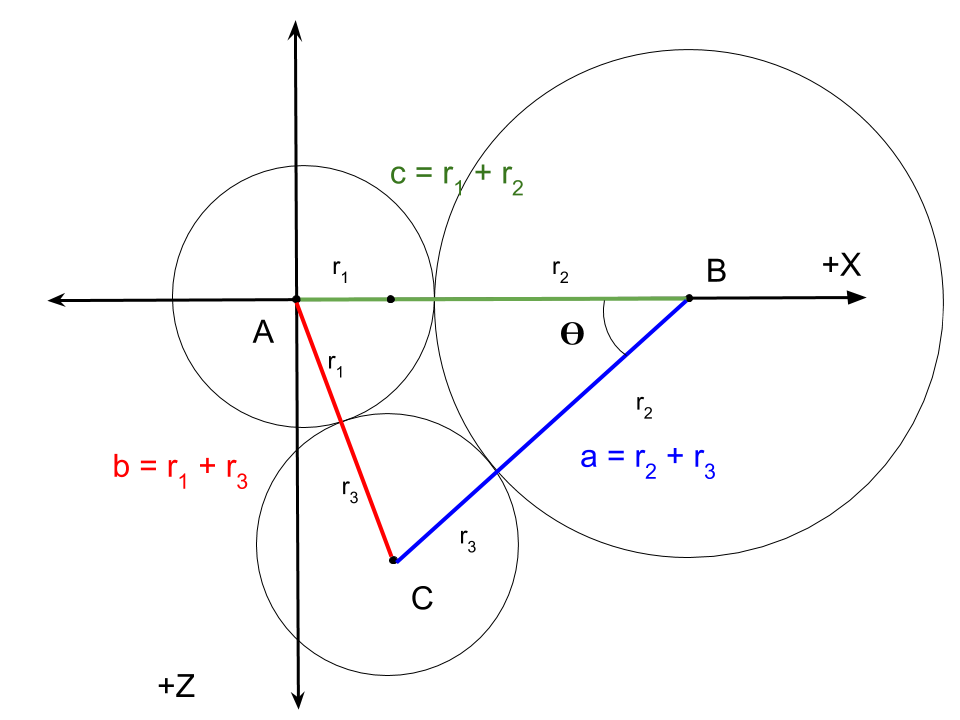
\includegraphics[width=0.5\textwidth]{figures/ThreeTouchingCircles.png}
     \caption{Three Touching Circles}
  \label{fig:Tangent}
\end{figure}

To solve this problem most conveniently, we place the first circle on the negative $x$-axis, and the second circle
on the positive $x$-axis, with the circles intersecting at the origin.
The third circle is place in the positive $y$ direction. It's center will not be on the $y$-axis itself unless the
radii of the first two circles are equal.

We seek a formula for the coordinates of the third circle in terms of three input radii $r_1,r_2,r_3$.

Because the distance between adjacent circles is the sum of their radii, define:
\begin{align}
a  &= r_2 + r_3 \\
b  &= r_1 + r_3 \\
c  &= r_1 + r_2
\end{align}

Then we can use the cosine law to compute the angle $\angle ABC = \theta$:


\begin{align}
  \theta  &= \arccos{\frac{a^2 + b^2 - c^2}{2bc}} \\
  \theta  &= \arccos{\frac{(r_2+r_3)^2 + (r_1+r_3)^2 - (r_1+r_2)^2}{2(r_1+r_3)(r_1+r_2)}} \\
\end{align}

It is clear that once $\theta$ has been calculated:

\begin{align}
 C_z  &= a\sin{\theta}
\end{align}
Allowing us to form a right triangle $\triangle ACD$ and use the Pythagorean theorem:
\begin{align}
  b^2  &= C_z^2 + C_x^2 \\
  C_x   &= \sqrt{b^2 - C_z^2}  \\
\end{align}




\section{Three Touching Spheres}


Our fundamental goal now is to describe three touching spheres. As robotocists,
our interest is in the slope of the plane of the tops of these spheres
as if they were resting on a table. Then by inflating or deflating spheres,
we would be able to control the direction of a plane or platform.
Such a device is sometimes called a parallel manipulator, of which a
Stewart Platform\cite{wiki:stewart} (\url{https://en.wikipedia.org/w/index.php?title=Stewart_platform&oldid=898429010})
is the best-known example.

The fundamental action of a parallel manipulator is to tilt a plane or platform in a desired direction based
on changes in the radii of the spheres.

The problem finding the planes tangent to three touching spheres
is given as an exercise in an advanaced textbook on solid geometry from 1881\cite{payne1881}. It does not give a solution, but it gives a hint: to consider the cones enveloping
three spheres taken two at a time.

Choosing the coordinate system of the $XZ$ plane through the center of the spheres greatly
simplifies the derivations, because the center of the spheres always form tangent circles
in this plane. Call this plane the {\em center plane.} The position of $A$ is fixed, $B$ is constrained to the $x$-axis, and
$C$ is contrained to the $xz$-plane. The center of these circles in the $xz$ plane can be
calculated from the radii independent of the tilt they induce.
In this coordinate system, the $y$-coordinate of the center of all spheres is $0$.
Furthermore, a cone tangent to two spheres has its axis and apex in the $xz$-plane.
The projection of all three spheres into this plane produces three touching circles.
We seek an expression for the normal of the plane of the tops of these spheres as a function
purely of the three radii. Call this plane the {\em top plane}.
We can imagine the spheres resting on a fixed surface called the {\em bottom plane}.
The tilt of the top and bottom plane relative to the center of the spheres
is alway a mirror image of each other across the coordinate $XZ$-plane.

If the tilt of the top plane relative to the coordinate plane is given by a rotation about the $z$ axis of $\theta$ and
then a rotation about $x$ axis of $\gamma$, the tilt of the top plane relative
to the bottom plane is given by the $zx$ extrinsic Euler angles $(2\theta, 2\gamma)$.

\subsection{Physical Embodiment}

To embody this system precisely, the sphere $A$ could be pinned to
the origin of the bottom plane.
The contact point of the sphere $B$ with the bottom plane could be placed on a
linear slider on the $x$-axis. The conact point $C$ could be constrained to
rest on the botom plane by gravity or some elastic cables. As the spheres
change change, the origin of the center plane will experience minor translation
relative to the bottom plane, but will not experience rotation about the $y$-axis.
If needed the coordinates of the spheres in the bottom plane can be easily
calculates from the radii and the computed Euler angles $\theta$ and $\gamma$.

\begin{figure}
     \centering
     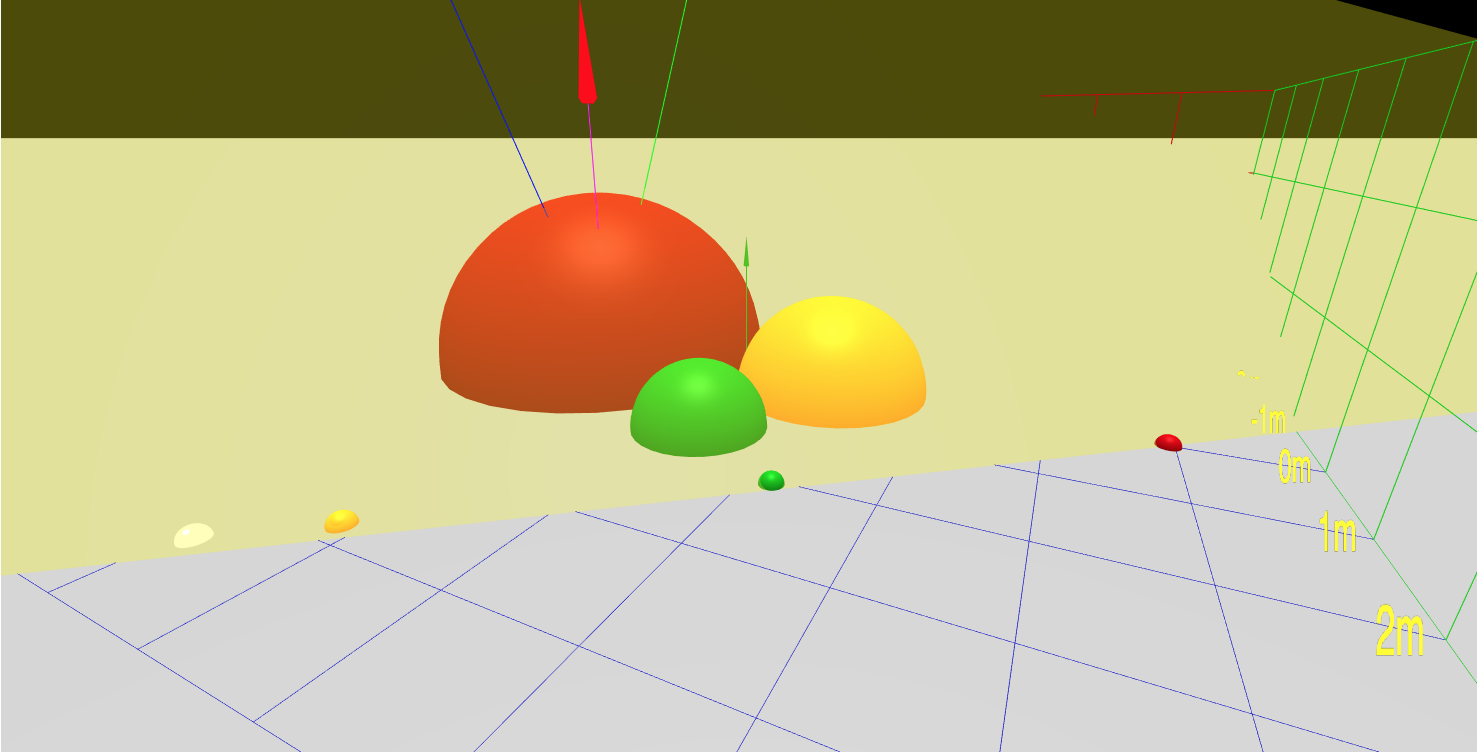
\includegraphics[width=0.99\textwidth]{figures/StandardThreeSphereDiagram.png}
     \caption{Three Touching Spheres}
  \label{fig:fixed}
\end{figure}

\subsection{Variable definitions}

We assume that the spheres centered at points $A,B,$ and $C$
of radii $r_A,r_b,$ and $r_c$. We setup our coordinate system as a right-
handed coordinate system with $XZ$ plane contaning the center of all spheres.
The $A$ sphere is placed at the origin, so that $O = A$, and the $B$ sphere
is place on the positive $X$ axis. Without loss of generality assume $r_a \geq r_b \geq r_c$.
Following computer graphics convention, we think of the $Y$ dimension as vertical.

Taking any two spheres defines a cone whose apex is in the $XZ$ plane.
Call the apex of the $AB$ cone $U$, the $AC$ cone $V$, and the $BC$ cone $W$.

It is a beautiful fact that the th apices $U,V$ and $W$ are colinear
on a line we call the {\em apex line}, depicted in both Figure \ref{fig:fixed}
or Figure \ref{fig:rotation}.
Further, by your choice of coordinates,
this line is in the $XZ$ plane. Finally, the top and bottom planes
intersect at this line, because those planes are tangent to the three cones.

We assert that these three points form a line, which we call the {\em apex line}, in the $XZ$ plane and that this
line is the intersection of the {\em tangent plane} touching all three spheres at a single point
with the $XZ$ plane. We will use points $U$ and $V$ in our calculation.

\subsection{Axis Angle of Cone Enveloping Two Spheres}

In order to compute the apex line, it is helpful
to note that the apex angle $\psi$ of a cone which envelopes (by being tangent to) two tangent
spheres of radii $r,s$, is:

\begin{align}
 \psi &= \arcsin{\frac{r s - r^2}{2 r^2 - r s + s^2}} \\
\end{align}
where $r < s$ without loss of generality. Note that when $r = s$
there is a special case,
the cone tangent to both is degenerate (that is, a cylinder, or a cone of
$\psi = 0$ apex angle.)

\subsection{Strategy}

We seek to compute the normal of the tangent plane.
Observe that this plane is tangent to all three cones.
Observe that the $AB$ cone intersects
the $A$ sphere in a circle on the surface of the $A$ perpendicular to and centered on the $X$ axis.

The half-angle of a cone tangent to two tangent spheres is computed from the radii directly:
\begin{align}
  \theta_{ab} &= \arcsin{\frac{r_a - r_b}{r_a + r_b}} \\
  \theta_{bc} &= \arcsin{\frac{r_b - r_c}{r_b + r_c}}
\end{align}


\begin{figure}
     \centering
     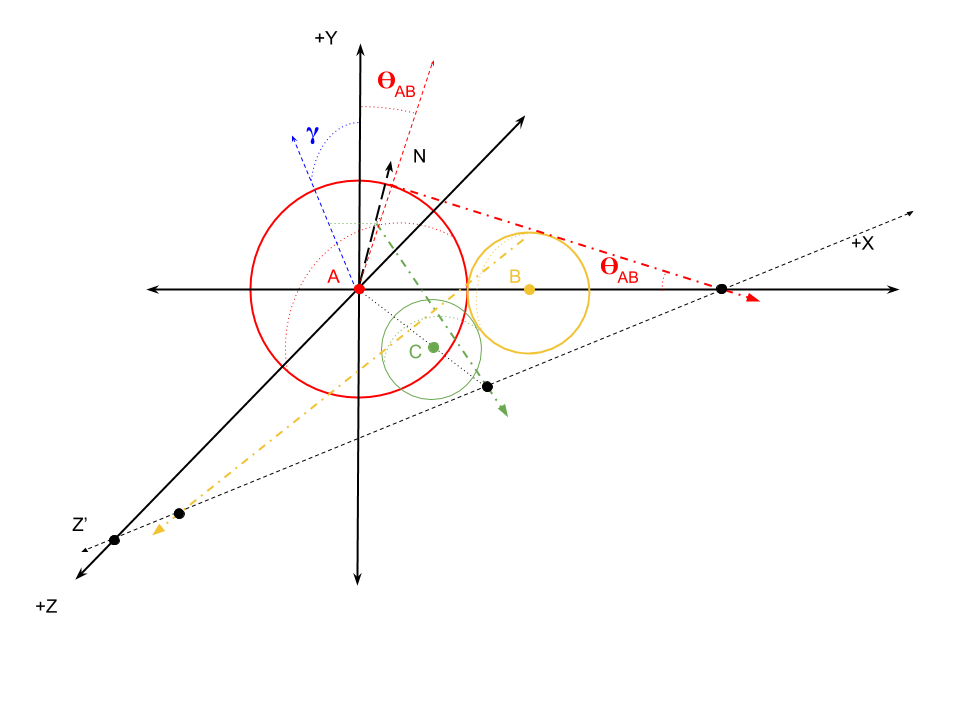
\includegraphics[width=0.5\textwidth]{figures/RotationMath.png}
     \caption{Rotation Math}
  \label{fig:rotation}
\end{figure}

A vector of length $r_A$ that is always rotated about the origin is always a point on the sphere.
The first operation is move this vector perpendicular to the $AB$ cone.
A vector $N$ in the $Y$ direction and rotated counterclockwise
about the $Z$-axis by $\theta_{ab}$ is perpendicular to the $AB$ cone.

However, we must rotate this vector $N$ about the $X$ axis by an unknown amount, $\gamma$, in order
to orient the vector to line up properly with the desired tilt of the tangent plane despite not being a pure rotation about the $Z$ axis. Since this angle is computed in the $YZ$ plane, we compute a projection of the point $V$ into
that plane, forming a triangle in the $YZ$ plane.  Call this point $I_z$, the intersection
of the apex line with the $Z$-axis. Let $h$ be the height of the intersection of the y-axis with the $AB$ cone.
Then $\gamma$ is the angle we need to rotate the plane by so that it intersects with the $Z$-axis at a point, referred to as $I_z$. By basic geometry of simialr triangles, this is computed from the right triangle of the origin with $h$ and $I_z$.
Having computed $\theta_{ab}$ and $\gamma$, these two degrees of rotation give us the plane tangent to all three spheres, and its corresponding tilt for our desired soft Stewart Platform.

Vectors $\overrightarrow{U}, \overrightarrow{V}, $ and $  \overrightarrow{W}$ represent the vectors from the center of the spheres $A$, $B$, and $C$ to
the apices of the cones tangent to $A$ and $B$, $B$ and $C$, and $C$ and $A$ respectively.


\begin{align}
  \overrightarrow{U} &= \overrightarrow{A} + \hat{\overrightarrow{AB}} \frac{r_a}{\sin{\theta_{ab}}} \\
  \overrightarrow{V} &= \overrightarrow{B} + \hat{\overrightarrow{BC}} \frac{r_b}{\sin{\theta_{bc}}} \\
\end{align}

The point $H$ is the intesection of the $AB$ cone with the $y$ axis.
This is right triangle of the origin with the points $U$ and $H$. (The hypotenuse
of this triangle is $\overrightarrow{HU}$, and side adjacent to $\theta_{AB}$ is $\overrightarrow{OU}$.)
It is computed by projecting the contact point of the top plane in the $xy$-plane
onto the $xz$-plane. This allows $\gamma$ to be computed as a pure rotation
about the $x$-axis.

\begin{align}
H_y &= U_x\tan{\theta_{ab}}\\
z' &= \frac{U_xV_z}{U_x - V_x} \\
\gamma &= \arcsin{\frac{H_y}{z'}}
\end{align}









\bibliographystyle{acm}

\bibliography{softrobotmath}


\end{document}


  In 1881, the problem of computing the plane tangent to three spheres was set as an exercise in a textbook, {em Practical Solid Geometry}\cite{payne1881}. We have solved this problem in JavaScript, producing an interactive, browser-based web page that dynamically solves the problem. All of the code is released under the GNU Public License. We propose constructing a ``soft'' Stewart platform using this theory which  allows us to control the inclination of two planes with a very simple  mechanism powered only by phase change of a liquid to a gas or by pneumatics. Future work includes computing the Jacobian of a ``tentacle'' formed  by stringing together many such Stewart Platforms, thus providing a  theoretical model for a simple, inexpensive, ``soft'' tentacle.  Such a tentacle can be scaled down nicely for {\em in vivo} medical  applications such as endoscopy and arterial catheterization.


  \section{Thing to Research}

Idea: It may be possible to solve for the support points as the intersection of cones\cite{shene1994lower}.

Note problem CXLVIII (148). Page 195
Joseph Payne (of the Charterhouse)
``Practical solid geometry; or, Orthographic and Isometric projection.

http://www.coe.org/p/fo/et/thread=11194

https://math.stackexchange.com/questions/2101056/how-to-compute-the-formula-of-common-tangent-plane-of-three-spheres

https://math.stackexchange.com/questions/1129402/solving-a-common-tangent-problem-using-matrices


We used this derivation with Wolfram Alpha:
\begin{align}
 z &= -2 \frac{r_x^2}{r_x - r_y}\\
 \psi &= 2 \arcsin{\frac{r_x}{z + r_y}} \\
 \psi &= 2 \arcsin{\frac{r_x}{-2 \frac{r_x^2}{r_x - r_y} + r_y}} \\
 \psi &= \arcsin{\frac{r_x r_y - r_x^2}{2 r_x^2 - r_x r_y + r_y^2}} \\
\end{align}
